\documentclass{article}

\usepackage{Paper}
\pdftitle{Report MS-01-Initialization}

\begin{document}

\hypersetup{citecolor=black}

\begin{titlepage}
    \begin{wrapfigure}{l}{7.5cm}
        \hspace*{.01cm}
        
\includegraphics[width=.3\textwidth]{media/hslu-logo-2.png}

        \vspace*{.01cm}
        \hspace*{.16cm}
\includegraphics[width=0.4\textwidth]{media/hslu-svg-logo.png}
    \end{wrapfigure}

    \phantom{}
    \vspace*{-1cm}

    \begin{flushright}
        
\includegraphics[width=.225\textwidth]{media/tuefterpark_logo.png}
    \end{flushright}

    \wrapfill

    \vspace*{-3.5cm}
    {\huge \textbf{Waste management}}

    {\Large Milestone report 1: Initialization}

    \vspace*{3cm}
    \begin{center}
        {\Huge \textbf{Picture space}}
    \end{center}

    \vfill
    {\Large \textbf{Team 38}}\\[1em]
    \renewcommand{\arraystretch}{2}
    \begin{tabularx}{\textwidth}{>{\large}p{0.24\textwidth}>{\large}p{0.24\textwidth}>{\large}p{0.24\textwidth}>{\large}p{0.24\textwidth}}
    Blecha Antonin & Monti Antonio & Odermatt Patrick & Suvorova Maria \\
    Frongillo Matteo & Murali Arjun & Rosu Justin & von Fuchs Alexander
    \end{tabularx}
    \renewcommand{\arraystretch}{1}
    \vspace{.5cm}

    \large{\textbf{Coaches}: S. Züst, K. Dmitrjieva} 
    \vspace{.5cm}
    
    \large{\textbf{Submission date}: 10. October 2025}
\end{titlepage}

\newpage
\section*{Team 38}
\renewcommand{\arraystretch}{1.5}
\begin{tabular}{@{}p{0.19\textwidth}p{0.44\textwidth}p{0.3\textwidth}@{}}
\textbf{Name} & \textbf{Field of studies} & \textbf{E-mail} \\
Blecha Antonin & Energy and Environmental Systems Engineering & \href{mailto:antonin.blecha@stud.hslu.ch}{antonin.blecha@stud.hslu.ch} \\
Frongillo Matteo & Energy and Environmental Systems Engineering & \href{mailto:matteo.frongillo@stud.hslu.ch}{matteo.frongillo@stud.hslu.ch} \\
Monti Antonio & Energy and Environmental Systems Engineering & \href{mailto:antonio.monti@stud.hslu.ch}{antonio.monti@stud.hslu.ch} \\
Murali Arjun & Energy and Environmental Systems Engineering & \href{mailto:arjun.murali@stud.hslu.ch}{arjun.murali@stud.hslu.ch} \\
Odermatt Patrick & Energy and Environmental Systems Engineering & \href{mailto:patrick.odermatt@stud.hslu.ch}{patrick.odermatt@stud.hslu.ch} \\
Rosu Justin & Electrical Engineering & \href{mailto:justin.rosu@stud.hslu.ch}{justin.rosu@stud.hslu.ch} \\
Suvorova Maria & Energy and Environmental Systems Engineering & \href{mailto:maria.suvorova@stud.hslu.ch}{maria.suvorova@stud.hslu.ch} \\
von Fuchs Alexander & Electrical Engineering & \href{mailto:alexander.vonfuchs@stud.hslu.ch}{alexander.vonfuchs@stud.hslu.ch} \\
\end{tabular}

\vspace*{1cm}
%\begin{figure}[ht!]
%    \centering
%    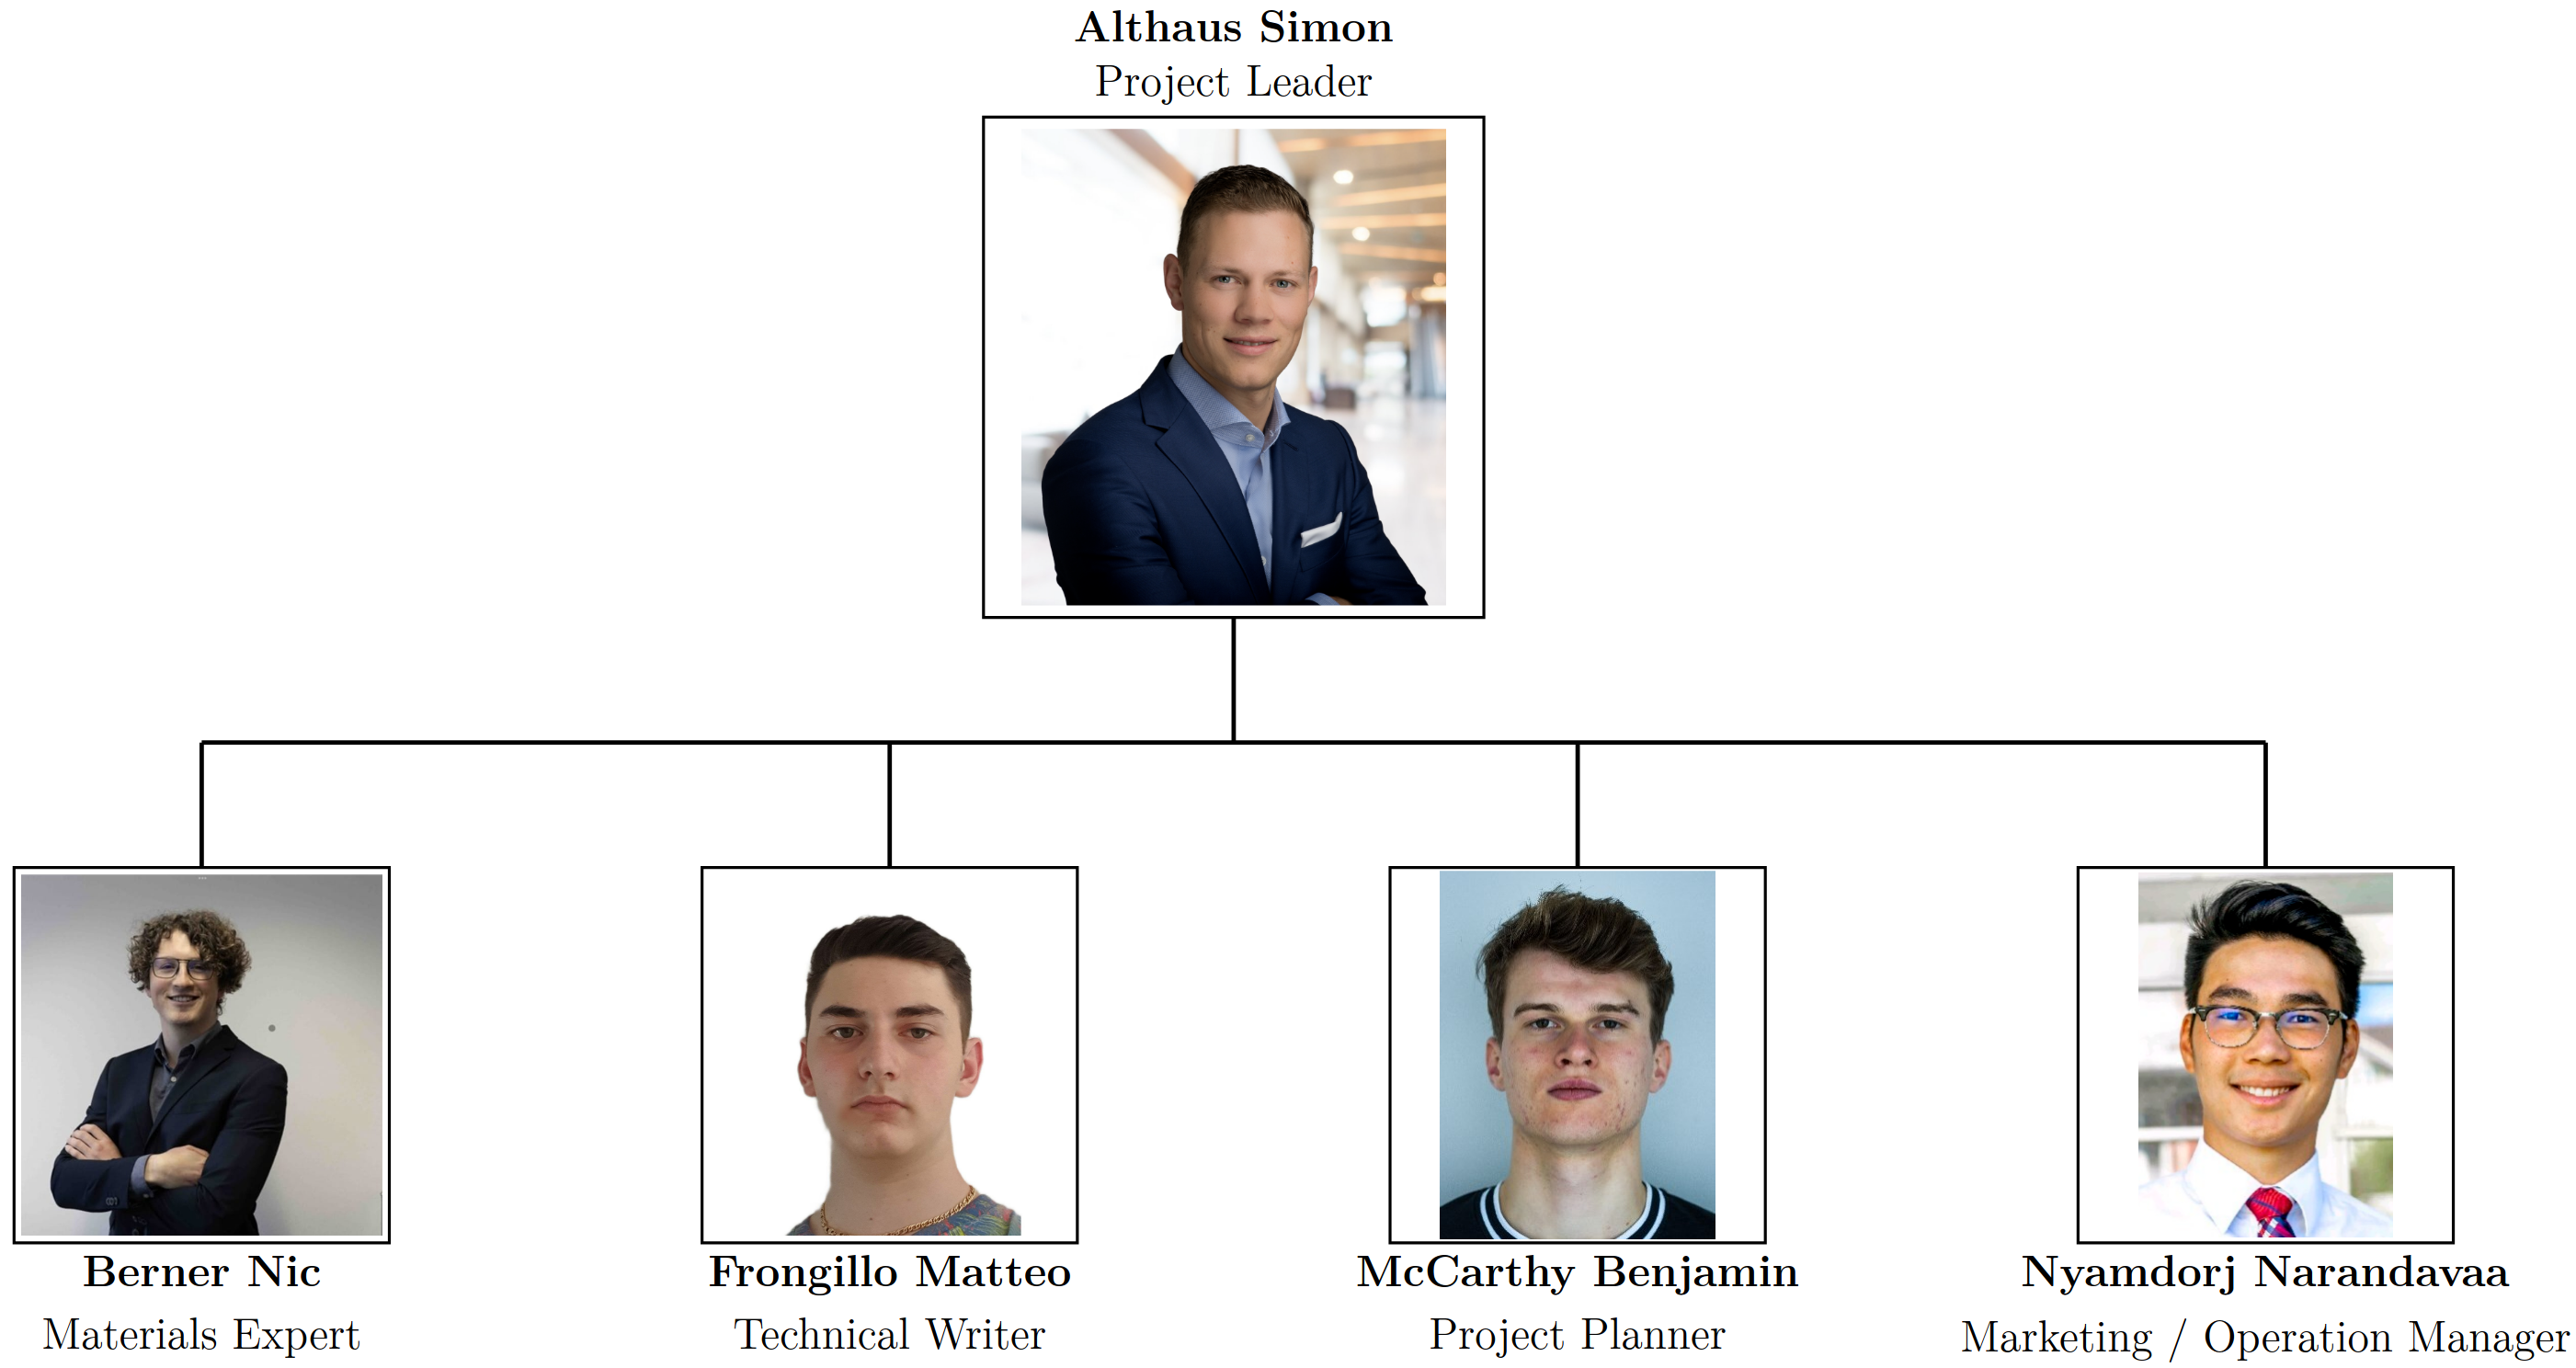
\includegraphics[width=\textwidth]{media/organisational_chart.png}
%    \caption{Organisational chart}
%    \label{fig:organisational_chart}
%\end{figure}

\newpage
\section*{Summary}
TODO
\newpage

\tableofcontents
\newpage

\section{Introduction}

\section{Process}
Concept Phase \& System Design (Rough Concept): Using creative and analytical methods, you will
systematically develop and evaluate three different solution concepts. These describe fundamental
approaches to how the tüftelPark-kit could essentially be realized. You will present these results to
the experts from the Tüftelpark.

\section{Functional components}
\subsection{Components}
The kit must be based on specific technical basis (TueftelPlattform).
The TueftelPlattform consists of:
\begin{itemize}
    \item Arduino Uno with Grove-Shield
    \item I2C motor driver board
    \item Power supply via 7.4V / 1300 mAh Li-Ion battery
    \item Freely selectable Grove sensors and actuators
    \item The mechanical components can be made from 4mm poplar plywood (CO$_2$ laser) and 3D-printed parts
    \item Optional components from the Stokys range are available
\end{itemize}

Standard components (e.g. connecting elements, bearings, ...) may also be used.

\section{Organisational components}
\subsection{Dimensions}
The system must be designed in such a way that it can be packed in a standard stacking
container measuring 60 x 40 x 32.3 cm during PDP and must not exceed a total weight of 20 kg. This
is necessary to ensure efficient and safe storage of the prototypes during the semesters.








\newpage
\section{References}

\appendix
\section{List of stuff}

\end{document}

